

\chapter{Graphics}

\begin{figure}[H]
\centering
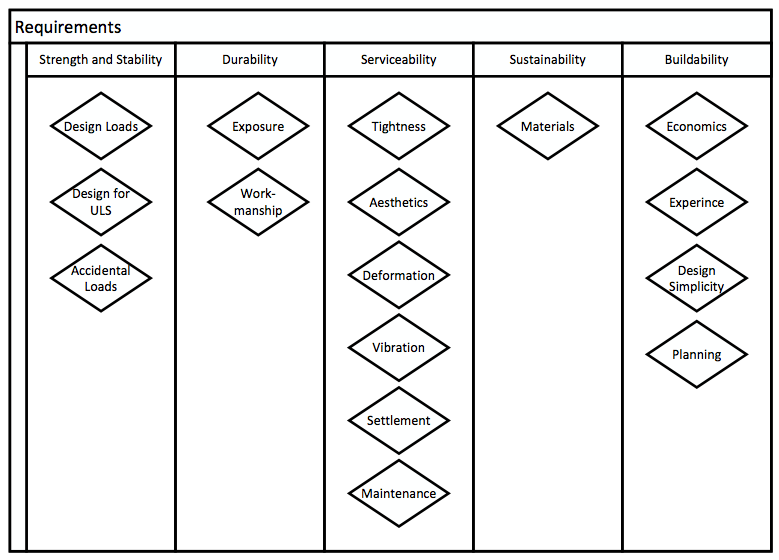
\includegraphics[scale=0.4]{img/GR-FR.png}
\caption{Functional requirements for Buildability.}
\label{figure:test}
\end{figure}


\section{Plots}
Plots are preferably done using the package \texttt{pgfplots}. Below is an example given. The example also show how to put figures side-by-side in your document using the \texttt{\textbackslash subfloat} command. Open \texttt{data.txt} in a text editor and have a look at its structure. The \LaTeX{} document reads the data from the text file and produces a plot. Axes are automatically scaled depending on the data range given in the text file. 

%------------------------------------------------------------------------------------
\begin{figure}[H]
\centering
\subfloat[Diagonal components of $\bar{D}$.]{
\begin{tikzpicture}
\begin{axis}[
	scale=0.85, % size of the plot
	every axis/.append style={line width=1pt},
    xlabel = $\bar{\varepsilon}_\text{zz}$,
    ylabel style={align=center},
    ylabel = $D_\text{cp}$,
    y unit = {\si{\kilogram\per\meter\square\second}},
    x unit = -,
    cycle list name=linestyles,
    legend style={cells={anchor=west}},
    legend pos=north west,
    ]
\addplot table[mark=none,x expr=\thisrow{strain},y expr=\thisrow{Dxx}] {datafiles/data.txt};
\addplot table[mark=none,x expr=\thisrow{strain},y expr=\thisrow{Dyy}] {datafiles/data.txt};
\addplot table[mark=none,x expr=\thisrow{strain},y expr=\thisrow{Dzz}] {datafiles/data.txt};
\legend{$(\bar{D})_{xx}$,$(D)_{yy}$,$(D)_{zz}$};
\end{axis}
\end{tikzpicture}
\label{fig:a}
}\hfill % \hfill fills out the space inbetween the plots
\subfloat[Off-diagonal components of $\bar{D}$.]{
\begin{tikzpicture}
\begin{axis}[
	scale=0.85,
	every axis/.append style={line width=1pt},
    xlabel = $\bar{\varepsilon}_\text{zz}$,
    ylabel style={align=center},
    ylabel = $(\bar{D})_\bullet/D_\text{cp}$,
    ylabel style={yshift=-0.2cm},
    y unit = -,
    x unit = -,
    cycle list name=linestyles,
    legend style={cells={anchor=west}},
    legend pos=north west,
    ]
\addplot table[mark=none,x expr=\thisrow{strain},y expr=\thisrow{Dxy}] {datafiles/data.txt};
\addplot table[mark=none,x expr=\thisrow{strain},y expr=\thisrow{Dxz}] {datafiles/data.txt};
\addplot table[mark=none,x expr=\thisrow{strain},y expr=\thisrow{Dyz}] {datafiles/data.txt};
\legend{$(D)_{xy}$,$(\bar{D})_{xz}$,$(\bar{D})_{yz}$};
\end{axis}
\end{tikzpicture}
\label{thelabelcanbeanyingreally}
}
\caption{Components of the macroscale diffusivity tensor, $\bar{D}$, as a function of macroscale strain. Numerical values are normalized with respect to $D_\text{cp}$.}
\label{omg}
\end{figure}
%------------------------------------------------------------------------------------
You can cross-reference to each of the figures in this way: \cref{fig:a} and \cref{thelabelcanbeanyingreally}. You can also plot analytical functions \texttt{pgfplots} as shown in \cref{analytical} below.
%------------------------------------------------------------------------------------
\begin{figure}[H]
\centering
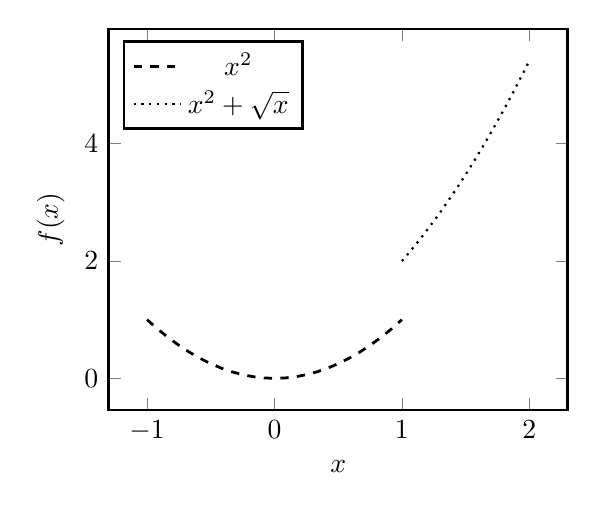
\begin{tikzpicture}
\begin{axis}[	scale=0.85,
every axis/.append style={line width=1pt},
xlabel = $x$,
ylabel = $f(x)$,
legend pos=north west,
]
\addplot[dashed,domain=-1:1]{x^2};
\addplot[dotted,thick,domain=1:2]{x^2 + sqrt(x)};
\legend{$x^2$,$x^2 + \sqrt{x}$}
\end{axis}
\end{tikzpicture}
\caption{Examples of analytical functions.}
\label{analytical}
\end{figure}
%------------------------------------------------------------------------------------
